\section{Bevezetés}

Napjainkban egyre inkább terjednek el a különféle drónok, távirányítással vagy
akár önálló módon repülő többrotoros kopterek formájában. Számos nagyobb gyártó is
kínál a fogyasztói piacon készen megvásárolható termékeket, továbbá számtalan
lelkes ember áll neki otthon kísérletezni ilyesmi szerkezetek építésével.

Az ELTE biológiai-fizikai tanszékével szoros együttműködésben a Collmot kft.
rendelkezik körülbelül 40 saját építésű kopterrel, amelyeken az alacsonyabb szintű
motorvezérlő pilótaprogram felett belső feljesztésű rendszerük fut.

A szóban forgó drónok felhasználása igencsak változatos. Kutatási oldalról
például különböző tudományos szimulációk tesztelésére is alkalmasak, mint
mondjuk madarak vagy halak viselkedésének modellezése mesterséges neurális
hálók evolúciójának segítségével. Ezen felül szolgálhatnak továbbá
látványelemként is egy előre betáplált koreográfia útvonalának végigrepülése
közben LED lámpájuk fényerejét és színét változtatva.

\begin{figure}[h!]
  \center
  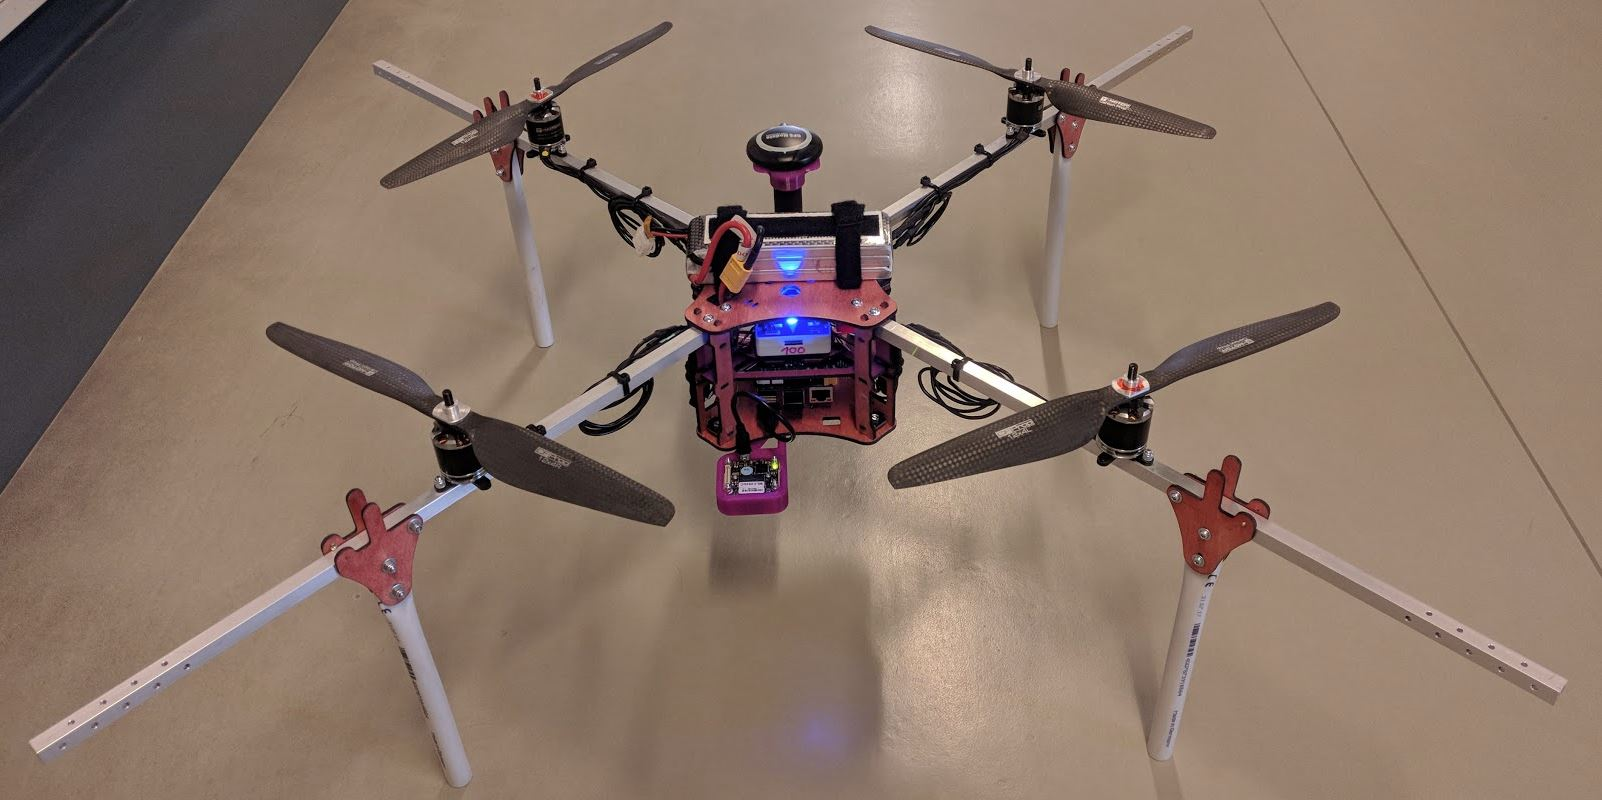
\includegraphics[width=0.8\textwidth]{drone.jpg}
  \caption{Fénykép a fent említett kopterek egy példányáról}
  \label{fig:drone}
\end{figure}

A FlockWave szoftver ötlete az ezen drónok monitorozására és vezérlésére készült
régebbi GroundControl nevű parancssori eszköz (lásd \ref{fig:groundcontrol}.
ábra) grafikus megjelenítéssel rendelkező megoldásra történő leváltásának
céljával fogalmazódott meg.

% TODO: Két mondatba?

\begin{figure}[H]
  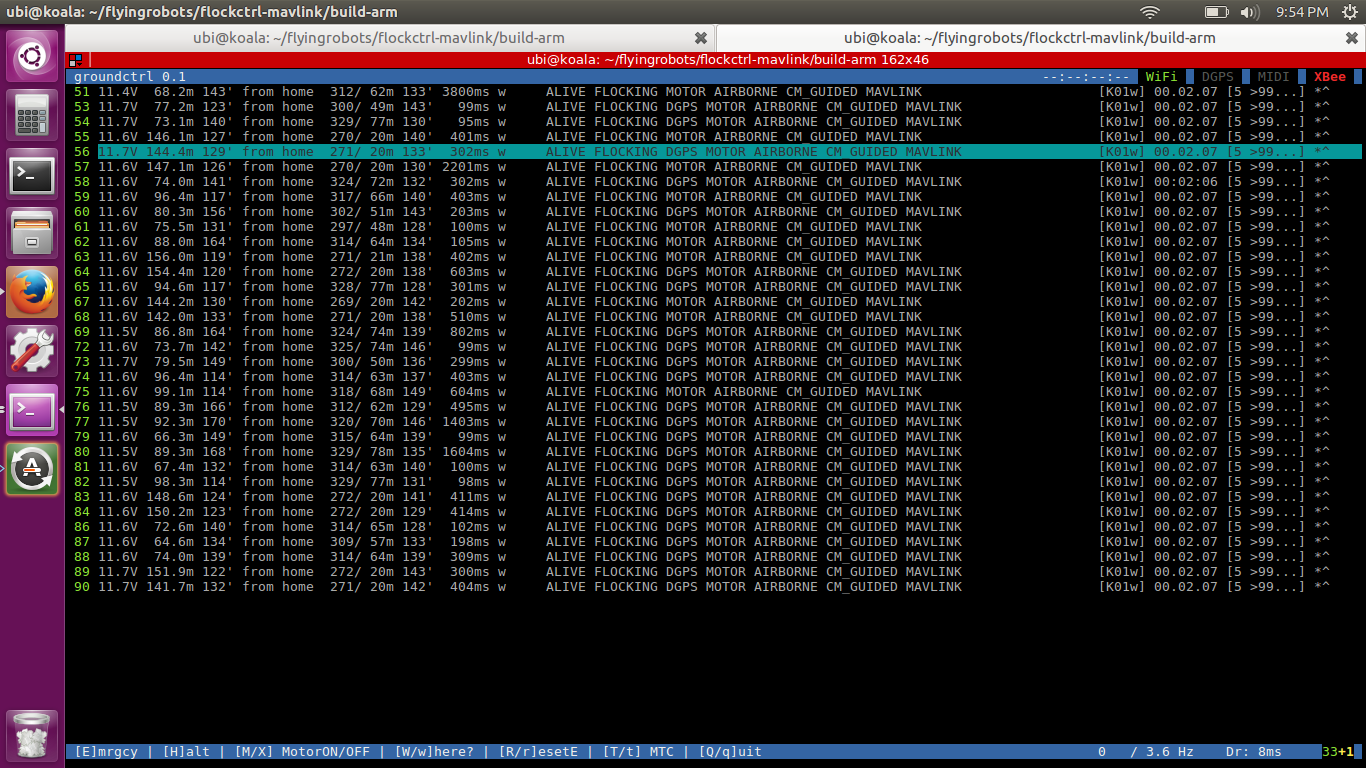
\includegraphics[width=\textwidth]{groundcontrol.png}
  \caption{Képernyőfotó a lecserélésre szánt régi karakteres kezelőfelületről}
  \label{fig:groundcontrol}
\end{figure}

\noindent Ennek az ötletnek a megvalósítási folyamatába
kapcsolódtam be még abban a kezdeti szakaszban, amikor a program körülbelül csak
a drónok pozícióját tartalmazó szerverről érkező csomagok feldolgozására és az
ezekből származó adatok alapján történő térképen való megjelenítésére volt
alkalmas. Ekkor lett a feladatom a rendszer további kiegészítő funkciókkal
történő ellátása. Ezek közül néhányat mutatok be kiemelve ebben a
szakdolgozatban.
